\documentclass[11pt,a4paper]{article}
\usepackage[T1]{fontenc}
\usepackage[ngerman]{babel}
\usepackage{amsmath}
\usepackage{parskip}
\usepackage{graphicx}
%\usepackage{listings}
\usepackage{hyperref}
\usepackage{float}

%opening
\author{Simon Cholewa}
\title{12. Clustering Exercise}

\hyphenation{
	Mo-tor-ü-ber-wach-ung 
}


\begin{document}

\maketitle

\section*{Exercise 1}

\subsection*{A) What is the best k?}
\begin{figure}[h!]
	\centering
	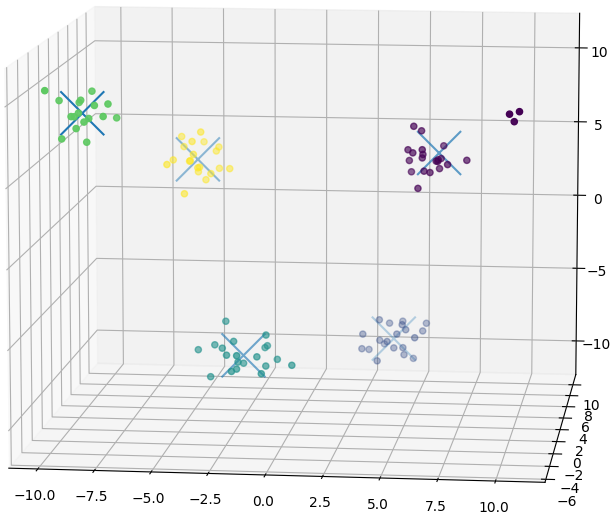
\includegraphics[width=0.9\linewidth]{Figure_3}
	\caption{Ein Scatterplot des Datensatzes. Es zeigt fünf Punktwolken. Die berechneten Schwerpunkte der Cluster sind mit Kreuzen gekennzeichnet. Die Zugehörigkeit der einzelnen Datenpunkte zu einem Cluster ist farblich kodiert.}
	\label{fig:scatterplot}
\end{figure}

Aus Abbildung \ref{fig:scatterplot} folgt, dass das optimale $k=5$ ist.


\subsection*{B) Can you print the clustering vector?}

Abbildung \ref{fig:scatterplot2d} zeigt die Entscheidungsgrenzen (\textit{clustering vectors}) zwischen den fünf Clustern. Die Grenze ist der Übergang zwischen jeweils zwei Farben.

\begin{figure}[h!]
	\centering
	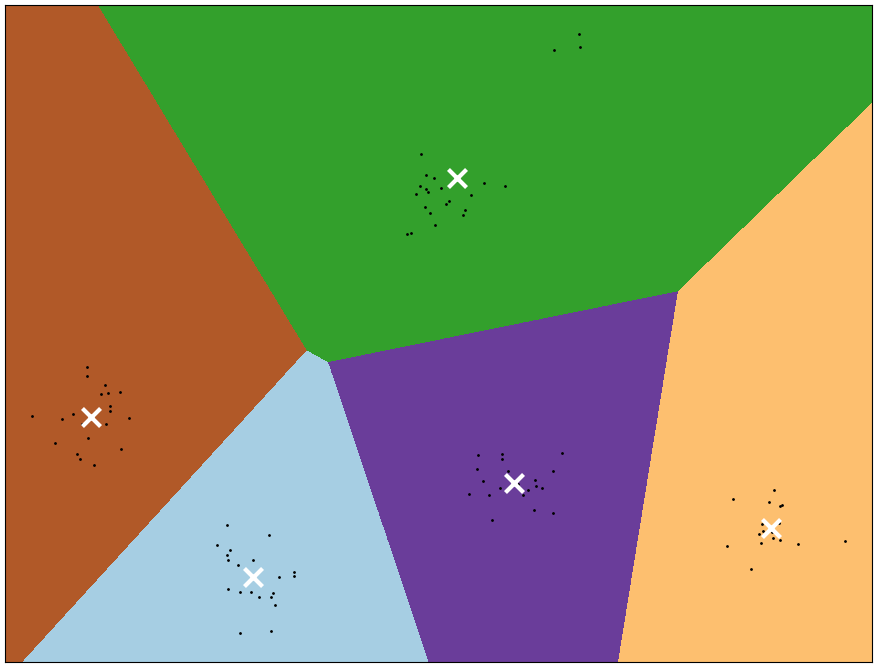
\includegraphics[width=1\linewidth]{Figure_4}
	\caption{Der dreidimensionale Datensatz wurde mittels PCA auf zwei Dimensionen reduziert, um die Grenzen zwischen den Clustern besser darstellen zu können. Die berechneten Schwerpunkte der Cluster sind mit Kreuzen gekennzeichnet. Die Zugehörigkeit der einzelnen Datenpunkte zu einem Cluster ist farblich kodiert.}
	\label{fig:scatterplot2d}
\end{figure}

\end{document}
